\documentclass[12pt]{report}

\usepackage[italian]{babel}
\usepackage[latin1]{inputenc}
\usepackage{url}
\usepackage{biblatex}
\usepackage{amsmath}
\usepackage{graphicx}
\usepackage{caption}


\bibliography{bib}

\title {IaasFog}
\author{Stefano Cadario, Luca Cavazzana}
\data{\date}

\begin{document}
\maketitle

\tableofcontents

\chapter{Introduzione}

\noindent bla bla bla bla

\chapter{Qualche titolo}

\section{Tracking delle features}

\noindent Crossratio, controllo sulla direzione, bla bla bla \dots

\section{Calcolo vanishing-point}

\noindent Ribla, ribla, ribla, \dots

\section{Calcolo del tempo all'impatto}

\noindent Dato un set di punti di coordinate $A$ e $B$, rappresentante una stessa feature in differenti immagini e conoscendo il framerate $f$ delle telecamera \`e possibile calcolare il tempo d'impatto, ossia l'istante in cui la feature attraverser\`a il piano immagine mediante il birapporto

$$ cross(i,a,b,v) = \frac{\overline{ia}}{\overline{ab}}\frac{\overline{av}}{\overline{iv}} = \frac{\overline{i'a'}}{\overline{a'b'}}\frac{\overline{a'v'}}{\overline{i'v'}} $$

\noindent Essendo nel mondo reale le distanze rispetto al vanishing point infinite, come quelle rispetto al piano della telecamera nelle immagini, la formula si semplifica

$$ \frac{\overline{ia}}{\overline{ab}} = \frac{\overline{a'v'}}{\overline{a'b'}} $$

\noindent Dal momento che $\overline{a'v'}$ e $\overline{a'b'}$ sono noti, ed essendo $ab$ la distanza percorsa dal veicolo fra le due immagini ($velocit\`a/framerate$), il tempo d'impatto pu\`o essere ottenuto come

$$ t_{i,b} = \frac{\overline{a'v'}}{\overline{a'b'}}\frac{\overline{ab}}{v} = \frac{\overline{a'v'}}{\overline{a'b'}}*f^{-1} $$

\section{Calcolo del contrasto}
\noindent Per il calcolo delle features sono stati presi in considerazione diversi approcci per il calcolo del contrasto nell'intorno di una feature: oltre alla formule di Michelson e Weber, gi\`a sfruttate nelle precedenti fasi del progetto, \`e stato deciso di introdurre anche Root Mean Square, che calcola il livello di contrasto secondo la formula

$$ c\left(I_{M\times N}\right) = \sqrt{\frac{1}{MN}\sum_{i=1}^N\sum_{j=1}^M(i_{ij}-\bar{I})^2} $$

\noindent Dal momento che nel calcolo del valore contribuiscono tutti i pixel all'interno della finestra tale formula risulta essere molto pi\`u resistente al rumore rispetto alle precendenti, il cui risultato risulta essere dipendente dall'errore sul singolo pixel centrale per Weber, e dall'errore sui valori di min e max per Michelson.\\
Confrontanto i valori ottenti calcolando i livelli di contrasto utilizzando i diversi metodi mostrano come RMS tenda a generare curve pi\`u smooth.

\begin{center}
	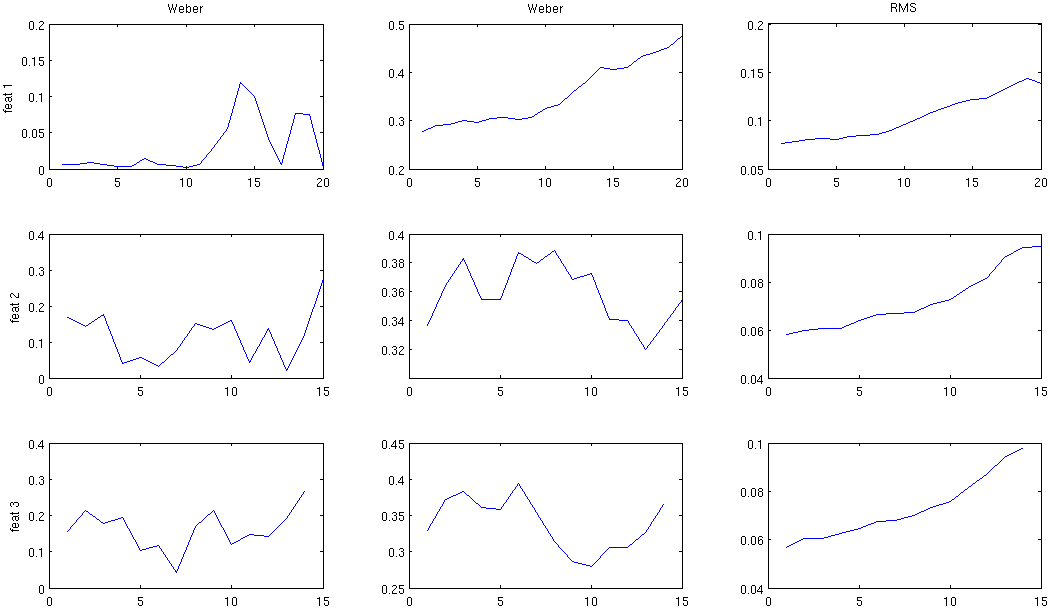
\includegraphics[scale=0.6, angle=90.0]{images/compContr1.png}
	\captionof{figure}{confronto fra i valori di contrasto ottenuti mediante i differenti approcci}
	\label{fig:contr01}
\end{center}
\begin{center}
	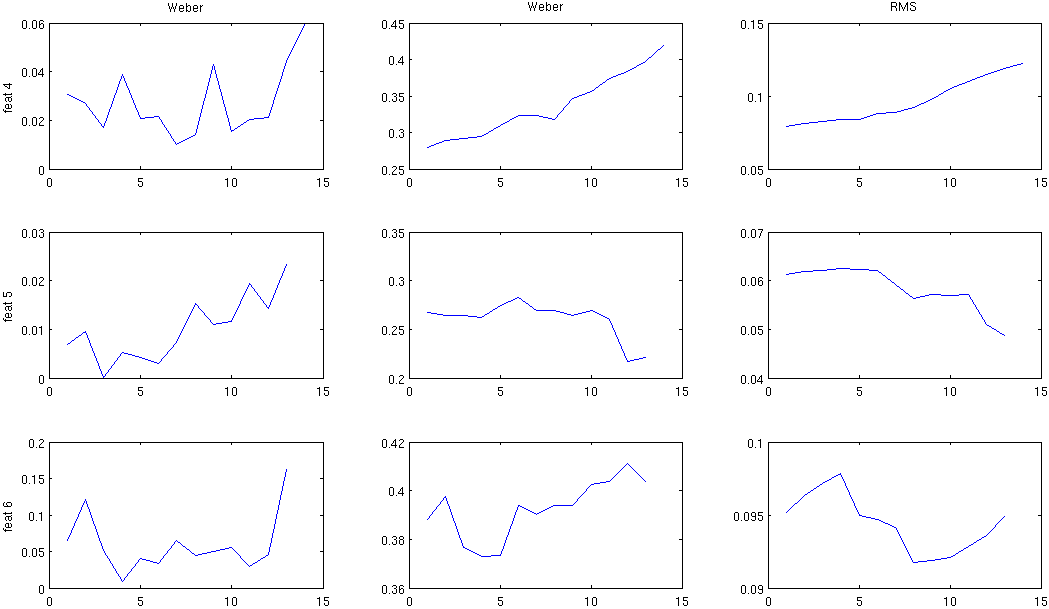
\includegraphics[scale=0.6, angle=90.0]{images/compContr2.png}
	\captionof{figure}{confronto su nuovi set}
	\label{fig:contr02}
\end{center}
\begin{center}
	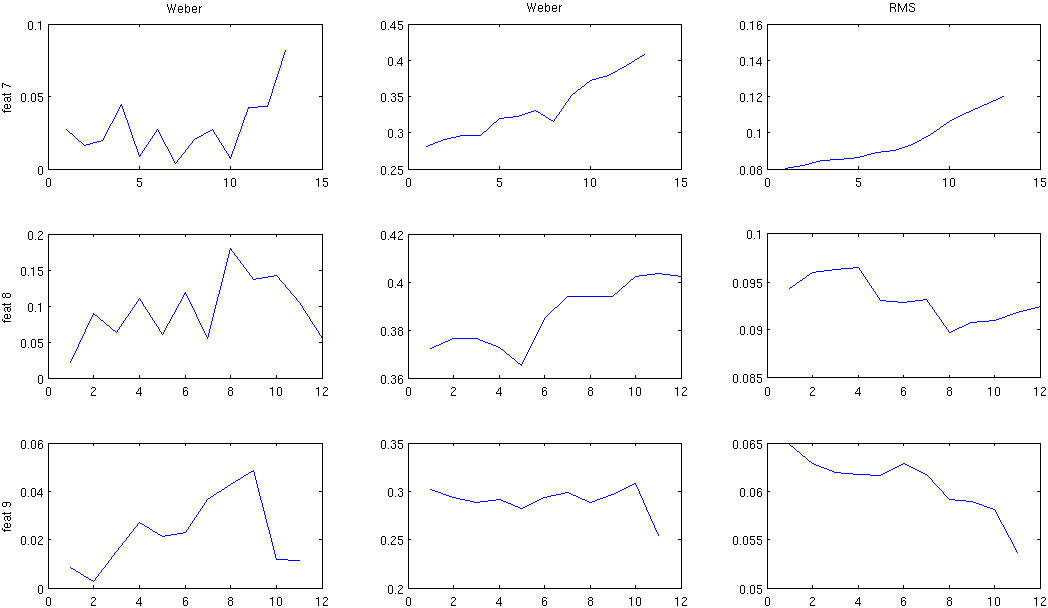
\includegraphics[scale=0.6, angle=90.0]{images/compContr3.png}
	\captionof{figure}{confronto su nuovi set}
	\label{fig:contr03}
\end{center}

\noindent Una particolarit\`a di RMS \`e che, al contrario delle altre tecniche, il risultato dipende dallo spazio di colori utilizzato per rappresentare l'immagine (facilmente aggirabile riscalando rispetto alla profondit\`a del colore).

\section{Stima dei parametri}

\subsection{Stima di $\lambda$ mediante minMax}

\noindent Definiamo la formula del contrasto per ogni feature come

$$ c_{i,s} = k_se^{-t_{i,s}/\lambda} $$

\noindent dove $c_{i,s}$ \`e il livello di contrasto all'istante $t_{i,s}$. Il parametro $k_s$ risulta essere costante all'interno di ogni singola sequenza di feature, mentre $\lambda$ \`e globale.
Sfruttando $k_s$ \`e possibile imporre la seguente uguaglianza fra due campioni nello stesso set

$$ c_1e^{t_1/\lambda} = c_2e^{t_2/\lambda} $$
$$ \lambda = \frac{t_2-t_1}{\log\frac{c_1}{c_2}} $$

\noindent in modo da stimare il parametro $\lambda$ sul singolo set utilizzando i livelli di contrasto massimi e minimi (ed i relativi tempi all'impatto).\\
A questo punto viene introdotto un primo semplice criterio atto ad eliminare set eccessivamente rumorosi: ricordando che i dati sono ordinati sul tempo d'impatto (e quindi il contrasto risulter\`a essere una funzione decrescente), vengono ignorati set in cui la differenza fra gli indici dei valori di contrasto minimo e massimo non \`e sufficientemente grande (nel nostro caso deve essere superiore alla met\`a del numero di feature all'interno del set).\\
Successivamente si pu\`o procedere con il calcolo di un $\lambda$ globale in base a quelli stimati calcolandone la media, mediana o applicando altre tecniche pi\`u complesse.

\subsection{Fitting di $\lambda$}
\noindent Una seconda tecnica adottata \`e stata quella di sfruttare la funzione \verb|fit| di Matlab per estrarre il parametro $\lambda_s$ che meglio descrive ogni singolo set di feature.\\
Funzioni particolarmente rumorose tendono a generare un $\lambda$ particolarmente elevato, portando ad una funzione che cresce rapidamente per poi appiattirsi subito sul valore di contrasto medio. Allo scopo di eliminare tali set vengono mantenuti solo quelli entro il quantile $0.8$ su $\lambda$.\\
I parametri dei singoli set vengono infine usati per stimare quello globale in modo simile al metodo precedente.

\subsection{Normalizzazione mediante fitting di $k$ e RANSAC}
\noindent Un'altra tecnica sperimentata consiste nello sfruttare tutte le informazioni disponibili  per stimare (mediante la funzione \verb|fit| di Matlab) i parametri $k_s$ e $\lambda_s$ che minimizzano l'errore su ogni singolo set di features.\\
$\lambda_s$, analogamente al metodo precedente, viene sfruttato per eliminare set eccessivamente rumorosi mantenendo solo quelli al di sotto del quantile $0.8$.\\
Il parametro $k_s$ viene invece utilizzato per normalizzare features con un valore di contrasto ``intrinseco'' (ovvero il massimo livello che otterremmo in condizioni idealei, senza nebbia): considerando $c_{i,s}/k_s$ possiamo cos\`i considerare sulla funzione discreta solo il contributo della nebbia, permettondoci di aggregare i dati di diversi set e stimare il parametro $\lambda$ globale sulla formula $$ c(t) = e^{-t/\lambda} $$ mediante RANSAC.\\
Questa implementazione di RANSAC seleziona a caso il $25\%$ dei set disponibili, i cui valori di contrasto vengono aggregati, ordinati in base al tempo d'impatto ed infine usati per stimare il $\lambda$ globale. Per tale parametro verrà poi calcolato il set di consenso ed il relativo errore, iterando il processo come da manuale.

\subsection{Confronto}
\noindent I test mostrano come il $\lambda_s$ sul singolo set di features ottenuto mediante minMax sia molto vicino a quello ottenuto mediante fitting in caso di campioni smooth (bella forza\dots), mentre per set pi\`u rumorosi (in verit\`a a contare \`e esclusivamente il rumore sui valori estremi) si ottiene una sottostima del valore (causato da un aumento della divergenza fra i valori massimo e minimo che portano ad un incremento del denominatore nella formula).\\
Gli approcci che fanno uso del fitting risultano essere invece molto pi\`u precisi, dal momento che sfruttano tutte le informazioni sull'intero set di dati, ma come prevedibile pagano un prezzo molto maggiore in termini di complessit\`a di calcolo.



\chapter{Funzioni}

Viene qui presentata una panoramica delle funzioni realizzate. Per informazioni pi\`u dettagliate circa il loro utilizzo consultare l'\verb|help| delle funzioni~\cite{lucaskanade81}.

\section[C++]{C\verb_++_}

\paragraph*{\verb_FindFeatures:_} main, parsa input e lancia nuFindFeatures

\paragraph*{\verb_nuFindFeatures:_} bla bla bla

\paragraph*{\verb_iaasFindCorners:_} estrae i corner dall'immagine

\paragraph*{\verb_iaasTrackCorners:_} cerca di rintracciare i corner della prima immagine (gi\`a calcolati) nella seconda

\paragraph*{\verb_verifyNewFeatureIsOk:_} verifica che una sequenza di corner sia coerente in base a \dots

\paragraph*{\verb_getAroundContrast:_} calcola il contrasto nell'intorno di una features usando RMS: $$ c\left(I_{M\times N}\right) = \sqrt{\frac{1}{MN}\sum_{i=1}^N\sum_{j=1}^M(i_{ij}-\bar{I})^2} $$

\paragraph*{\verb_verifyValidFeature:_} \dots


\paragraph*{\verb_printFeatures:_} scrive sul file la lista di feature valide come:
\begin{verbatim}
	     primoFrame numeroFrame [xCoord yCoord contrasto]+
\end{verbatim}

\section{Matlab}

\paragraph*{\verb_iaas:_}

\paragraph*{\verb_inspectContrast:_} stampa a video le sequenze di features per un'ispezione visiva

\paragraph*{\verb_myRansac:_} implementazione di RANSAC per calcolare il parametro lambda della funzione del contrasto dati in ingresso dei set di features normalizzati.






\paragraph*{\verb_fogLevel:_} date le coordinate del punto di fuga calcola il livello della nebbia come il livello di grigio medio nell'intorno se questi \`e omogeneo.

\paragraph*{\verb_MichelsonContrast:_} date le coordinate di una feature e la relative immagine restituisce il livello di contrasto nell'intorno come $$c\left(I\right) = \frac{\max(I)-\min(I)}{\max(I)+\min(I)}$$

\paragraph*{\verb_rsmContrast:_} date le coordinate di una feature e la relativa immagine calcola il livello di contrasto nell'intorno come $$ c\left(I_{M\times N}\right) = \sqrt{\frac{1}{MN}\sum_{i=1}^N\sum_{j=1}^M(i_{ij}-\bar{I})^2} $$

\paragraph*{\verb_WeberContrast:_} date le coordinate di una feature e la relative immagine calcola il livello di contrasto come $$c\left(i_{i,j}\right)= \frac{i_{i,j}-I_b}{I_b}$$ dove $I_b$ \`e il livello della nebbia, calcolato come il valore medio del frame.

\paragraph*{\verb_normContrast:_} normalizza il contrasto di ogni set di features utilizzando diverse tecniche:
\begin{itemize}
	\item \verb|first|: $ norm\left(c_i\right) = c_i/c_{1^{th}} $
	\item \verb|firstLast|: $ norm\left(c_i\right) = \frac{c_i-c_{n^{th}}}{c_{1^{th}} - c_{n^{th}}} $
	\item \verb|max|: $ norm\left(c_i\right) = c_i/c_{max} $
	\item \verb|minMax|: $ norm\left(c_i\right) = \frac{c_i-c_{min}}{c_{max} - c_{min}} $
	\item \verb|mean|: $ norm(c_i) = c_i/2\bar{c} $
	\item \verb|fit|: $ c_i / mle_{k}(\underline{c}) $
\end{itemize}

\noindent Di fatto quella che ci interessa maggiormente \`e \verb|fit|, le altre invece sono principalmente dei tentativi di approccio che non hanno avuto seguito nel progetto.

\chapter{Installazione}
\section{OpenCV}
OpenCV (Open Source Computer Vision) \`e una libreria di funzioni per la computer vision, inizialmente sviluppata da Intel e ora distribuita sotto licenza open source. \`E possibile scaricare l'ultima versione all'indirizzo \url{http://sourceforge.net/projects/opencvlibrary/} \footnote{guida d'installazione ufficiale all'indirizzo \url{http://opencv.willowgarage.com/wiki/InstallGuide}}.

\subsection{Windows}
Per compilare la libreria \`e necessario installare degli header offerti da MinGW (\url{http://http://www.mingw.org/}) e CMake (\url{http://www.cmake.org/cmake/resources/software.html}).\\
\noindent Una volta assicuratisi che il path dei binari di MinGW \`e fra le variabili di ambiente configurare OpenCV mediante l'interfaccia di CMake.

\subsection{Linux / MacOSX}

\noindent Per l'installazione \`e necessario disporre di \verb|cmake|, inoltre devono essere soddisfatte le seguenti dipendenze:
\begin{itemize}
\item \verb|ffmpeg|
\item \verb|libxine-ffmpeg|
\item \verb|libavcodec-dev|
\item \verb|pgk-config|
\item \verb|libgtk2.0-dev|
\end{itemize}

\noindent reperibili mediante \verb|apt-get| o package manager.\\

\noindent Una volta scaricata e scompattata l'ultima versione di OpenCV (2.2.0 alla stesura del presente documento), creare una cartella dove verranno salvate le librerie configurate mediante \verb|cmake| e aprirla con una finestra di terminale. Nel nostro esempio la creeremo nella stessa cartella scompattata

\begin{verbatim}
	$ cd OpenCV2.2.0/
	$ mkdir release; cd release
\end{verbatim}

\noindent Lanciare quindi il comando

\begin{verbatim}
	$ cmake -D CMAKE_BUILD_TYPE=RELEASE -D CMAKE_INSTALL_PREFIX=/usr/local
	-D BUILD_PYTHON_SUPPORT=ON -D BUILD_EXAMPLES=ON ..
\end{verbatim}

\noindent per configurare la libreria. Il valore della flag \verb|CMAKE_INSTALL_PREFIX| sar\`a l'indirizzo in cui si vorr\`a poi installare OpenCV. Se i sorgenti non dovessero trovarsi nella directory superiore, sostituire i due punti con il path corretto.\\

\noindent A questo punto non rimane che compilare ed installare le librerie mediante i comandi

\begin{verbatim}
	$ make
	$ make install
\end{verbatim}

\noindent ed esportare il path nelle variabili di ambiente con il comando

\begin{verbatim}
	$ export LD_LIBRARY_PATH=/usr/local/lib/:$LD_LIBRARY_PATH
	$ sudo ldconfig
\end{verbatim}

\noindent Se invece si preferisce non installare le librerie, esportare direttamente il path 

\begin{verbatim}
	$ export LD_LIBRARY_PATH=<opencv_dir>:$LD_LIBRARY_PATH
	$ sudo ldconfig
\end{verbatim}

\noindent dove \verb|<opencv_dir>| \`e la cartella dove abbiamo compilato il le librerie, nel nostro caso \verb|~/OpenCV-2.2.0/release|.

\section{Installazione ed esecuzione del programma}
\noindent Il progetto \`e disponibile via SVN alla pagina \url{http://code.google.com/p/iaasfog}.\\
Importare i sorgenti nella cartella \verb|c++| in Eclipse, importare gli header delle funzioni di OpenCV mediante Project $\rightarrow$ Properties  $\rightarrow$ C\slash C\verb|++| Editor $\rightarrow$ Settings $\rightarrow$ GCC C\verb|++| Compiler $\rightarrow$ Directories aggiungendo il percorso \verb|/usr/local/include/| e sotto GCC C\slash C\verb|++| Linker $\rightarrow$ Libraries le librerie \verb|opencv_core|, \verb|opencv_video|, \verb|opencv_highgui| e \verb|opencv_imgproc| in \verb|/usr/local/lib| (o qualunque path sia stato utilizzato per l'installazione).\\
Compilare.\\

\noindent In Matlab aggiungere il path degli m-file ed assicurarsi che il percorso specificato dalla varibile \verb|exec_path| in \verb|iaas.m| corrisponda alla cartella dell'eseguibile del codice C\verb|++|.\\
Per eseguire il programma lanciare nella console di Matlab il comando \verb|iaas [#]|, dove \verb|#|, opzionale, non far\`a visualizzare nessuna finestra se assente o uguale a \verb|0|, se uguale a \verb|1| visualizzer\`a una serie di grafici che mostrano le curve fittate, mentre se uguale a \verb|2| mostrer\`a un numero maggiore di grafici (modalit\`a pensata principalmente per il debugging, l'eccessivo quantitativo di grafici rischia di risultare tedioso per l'utente).

\printbibliography

\end{document}
